 \documentclass{beamer}

\usetheme{MagdeburgFIN}
\usefonttheme{structurebold}
\usepackage{graphicx}
\usepackage{float}
\usepackage{url}
\usepackage{pdfpages}


\title{Kick-Off-Presentation. Build Your Own Octopus(OctopusDB)}
\author{Ali Hashaam, Ali Memon, Guzel Mussilova, Pavlo Shevchenko}
\date{April 25, 2017}
\institute{Scientific Project: Databases for Multi-Dimensional Data, Genomics and Modern Hardware}

\begin{document}

\begin{frame}[plain]
 \titlepage
\end{frame}

\begin{frame}
\frametitle{Table of Contents}
\tableofcontents
\end{frame}

\section{Introduction to the Topic}

\subsection{Motivation}
\begin{frame}
\frametitle{Motivation}
Modern enterprises need to pick the right DBMSs for their data managing problems.\\ \pause
\hspace{0.2 cm} 1. Use specialized solution for each application. \\ \pause
\hspace{0.5 cm} $\rightarrow$ costly due to licensing fees, integration overhead and DBA costs\\ \pause
\hspace{0.2 cm} 2. Use a single specialized DBMS for all applications. \\ \pause
\hspace{0.5 cm} $\rightarrow$ compromise heavily on performance.
\footnote{A. Jindal. The Mimicking Octopus: Towards a one-size-fits-all Database Architecture, 2010}
\end{frame}

\subsection{Idea of OctopusDB}
\begin{frame}
\frametitle{Idea of OctopusDB}
Create a new type of database system without fixed store that will mimic several existing systems. \\ \pause
\begin{itemize}
\item{Storage Views}
\end{itemize}
Like "real" octopus can mimic other creatures and adjust to the environment
\end{frame}

\begin{frame}
\frametitle{Idea of OctopusDB}
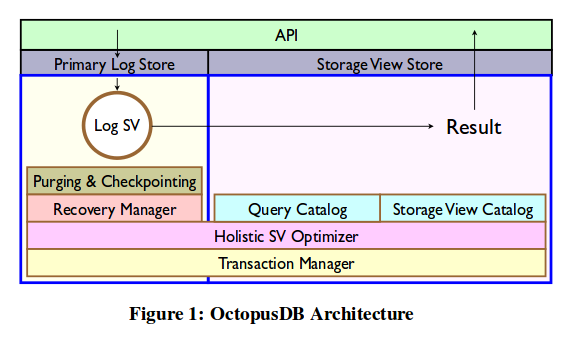
\includegraphics[scale=0.5]{img/octopus_arch.png}
\footnote{A. Jindal. The Mimicking Octopus: Towards a one-size-fits-all Database Architecture, 2010}
\end{frame}

\subsection{Our Goal}
\begin{frame}
\frametitle{Our Goal}
\begin{itemize}
\item{Not to \textbf{clone} OctopusDB} \pause
\item{Provide a \textbf{framework} that gives user a chance to act as \textit{Holistic SV Optimizer} and evaluate the results}
\end{itemize}
\end{frame}

\subsection{Our Vision}
\begin{frame}
\frametitle{Our Vision}
\end{frame}

\section{Project Organisation}

\subsection{Schedule}
\begin{frame}
\frametitle{Project Organisation.Schedule}
\textbf{Milestones} \\
\vspace{0.5 cm}
\begin{tabular}{|c|c|}
\hline 
02.05.2017 & MS-I (Kick-Off) \\ 
\hline 
23.05.2017 & MS-II (Concepts) \\ 
\hline 
13.06.2017 & MS-III (Implementation) \\ 
\hline 
04.07.2017 & MS-IV (Final) \\ 
\hline 
\end{tabular}
\\ \vspace{0.5 cm}
\textbf{Meetings} \\ 
\vspace{0.5 cm}
\hspace{0.5 cm} Team Meetings: Mo 14-15 \\
\hspace{0.5 cm} Meetings with supervisor: We 10-11

\end{frame}

\subsection{Roles}
\begin{frame}
\frametitle{Project Organisation.Roles}

\textbf{Team:} \\
\hspace{0.3 cm}Ali H. - \\
\hspace{0.3 cm}Ali M. - \\
\hspace{0.3 cm}Guzel - \\
\hspace{0.3 cm}Pavlo - \\

\vspace{0.2 cm}
\textbf{Supervisor:} \\
\hspace{0.3 cm} Gabriel Campero Durand \\

\vspace{0.2 cm}
Changing roles after each milestone.

\end{frame}

\begin{frame}
 \frametitle{Thank you for your attention! Any questions?}
\end{frame}

\section{Literature}
\begin{frame}
\frametitle{Literature}
\begin{enumerate}
\item{Jindal, Alekh. "The mimicking octopus: Towards a one-size-fits-all database architecture." VLDB PhD Workshop. 2010.}
\item{Dittrich, Jens, and Alekh Jindal. "Towards a One Size Fits All Database Architecture." CIDR. 2011.}
\item{Jindal, Alekh. "OctopusDB: flexible and scalable storage management for arbitrary database engines." (2012).}
\item{Idreos, Stratos, Martin L. Kersten, and Stefan Manegold. "Database Cracking." In CIDR, vol. 7, pp. 68-78. 2007.}
\item{Mozafari, Barzan. "Approximate query engines: Commercial challenges and research opportunities." SIGMOD, 2017.}
\end{enumerate}
\end{frame}


\end{document}
